\documentclass{beamer}
\usetheme{Boadilla}

\usepackage{amsmath}
\usepackage{amsfonts}
\usepackage{hyperref}

\usepackage{amsmath}
\DeclareMathOperator*{\argmax}{arg\,max}
\DeclareMathOperator*{\argmin}{arg\,min}

\title{Neural Architecture Search Using Deep Neural Networks and Monte Carlo Tree Search}
\author{Galina Boeva}
\institute{MIPT, 2024}


\begin{document}

\begin{frame}
    \titlepage
\end{frame}


\begin{frame}
    \tableofcontents
\end{frame}


\section{Motivation}
\begin{frame}{Motivation}
    \begin{block}{Main idea}
    NAS has demonstrated great success in automating the design of neural networks, but the prohibitively large amount of computing underlying NAS methods requires additional research to improve sampling efficiency and the cost of evaluating the network to achieve better results in less time.
    
    \end{block} 
    
\end{frame}


\section{AlphaX: A Scalable MCTS Design Agent}
\begin{frame}{AlphaX: A Scalable MCTS Design Agent}
%\centering
\begin{figure}
        \centering
        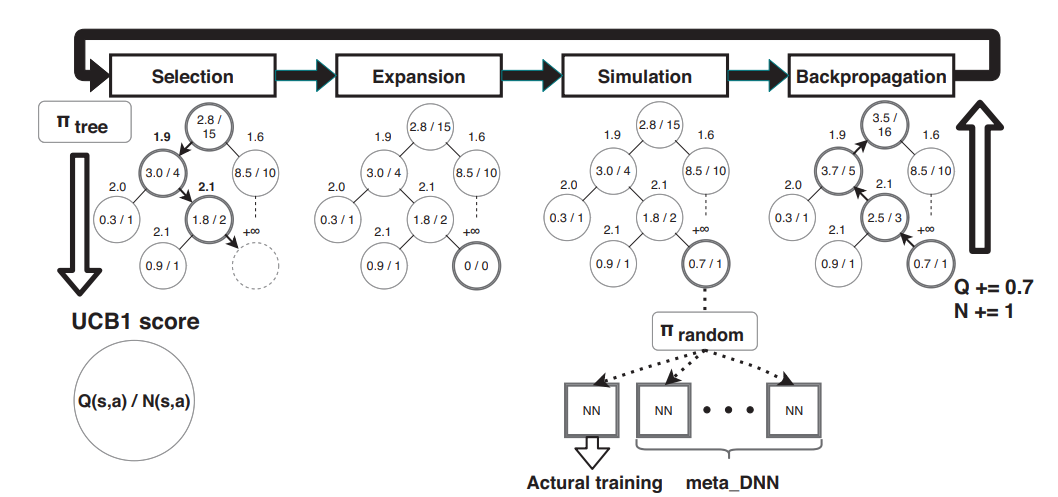
\includegraphics[scale=0.5]{images/nas2.png}
        %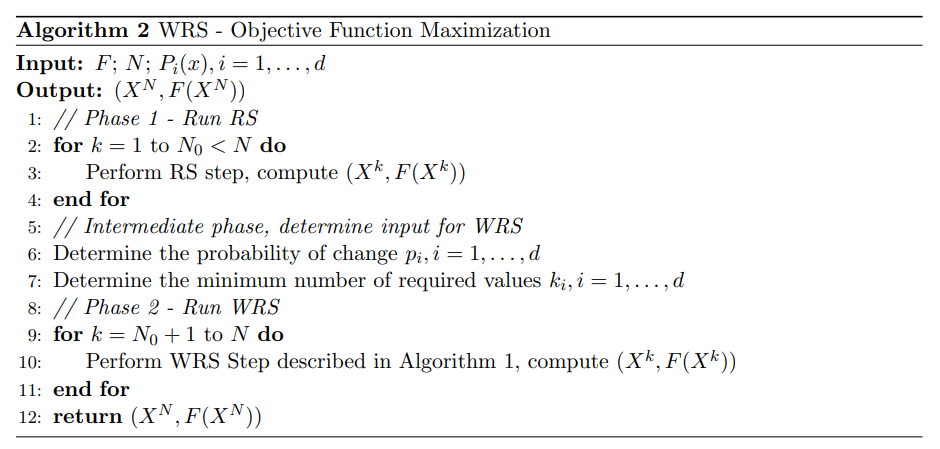
\includegraphics[scale=0.5]{images/wrs2.png}
        \caption{Overview of AlphaX search procedures.}
        \label{fig:enter-label}
    \end{figure}
\end{frame}
\begin{frame}{Design, State and Action Space}
%\centering
\begin{figure}
        \centering
        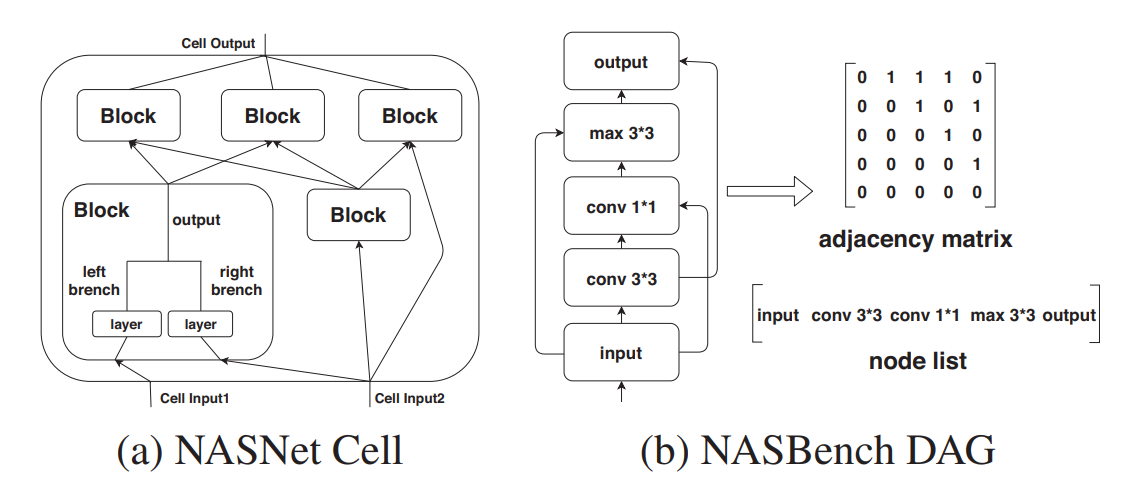
\includegraphics[scale=0.5]{images/nas3.png}
        %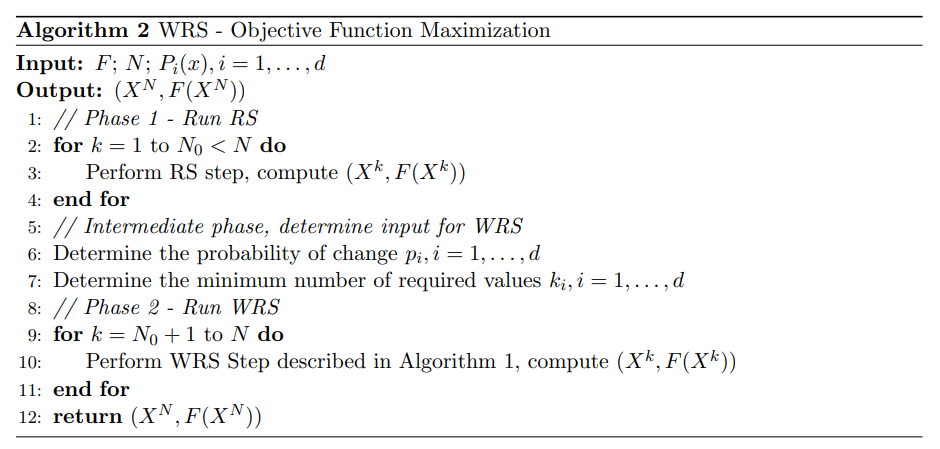
\includegraphics[scale=0.5]{images/wrs2.png}
        \caption{Design space: (a) the cell structure of NASNet and
(b) the DAG structure of NASBench-101. Then the network
is constructed by stacking multiple cells or DAGs.}
        \label{fig:enter-label}
    \end{figure}
\end{frame}

\begin{frame}{Search Procedure}
\begin{block}{Selection}
Moves down the search tree to trace the current most promising search path. It starts at the root and ends until it reaches the leaf. In the node, the agent selects actions based on UCB1:
$$\pi_{tree}(s) = \displaystyle \argmax_{a \in A} \left( \frac{Q(s, a)}{N(s, a)} + 2c
\sqrt\frac{2 \log N(s)}{N(s, a)}\right),$$
where $N(s)$ is the number of visits to the state $s$ (i.e. $N(s) = \sum_{a\in A} N(s, a)$), and $c$ is a constant.
\end{block}
\begin{block}{Expansion}
Adds a new node into the tree. $Q(s, a)$ and $N(s, a)$ are initialized to zeros. $Q(s, a)$ will be updated in the simulation step.
\end{block}
\end{frame}

\begin{frame}{Search Procedure}
\begin{block}{Meta-DNN assisted Simulation}
Randomly samples the descendants of a new node to approximate $Q(s, a)$ of the
node with their accuracies. 
$$Q(s, a) \gets \left(Acc(sim_{0}(s^{'})) + \frac{1}{k} \sum_{i=1\dots k} Pred(sim_{i}(s^{'}))\right) /2, $$
where $s = s + a$, and $sim(s)$ represents a simulation
starting from state $s$. Acc --- trained accuracy in the first simulation, Pred --- the predicted accuracy from Meta-DNN in subsequent $k$ simulations.
\end{block}
\begin{block}{Backpropagation}
Backtracks the search path from the
new node to the root to update visiting statistics. 
With the estimated q for the new node, we iteratively backpropagate the information to its ancestral as:
$$Q(s, a) \gets Q(s, a) + q, N(s, a) \gets N(s, a)+1, s \gets parent(s), a \gets \pi_{tree}(s)$$
\end{block}
\end{frame}



\begin{frame}{The design of Meta-DNN and its related issues}
\centering 
\begin{figure}
        \centering
        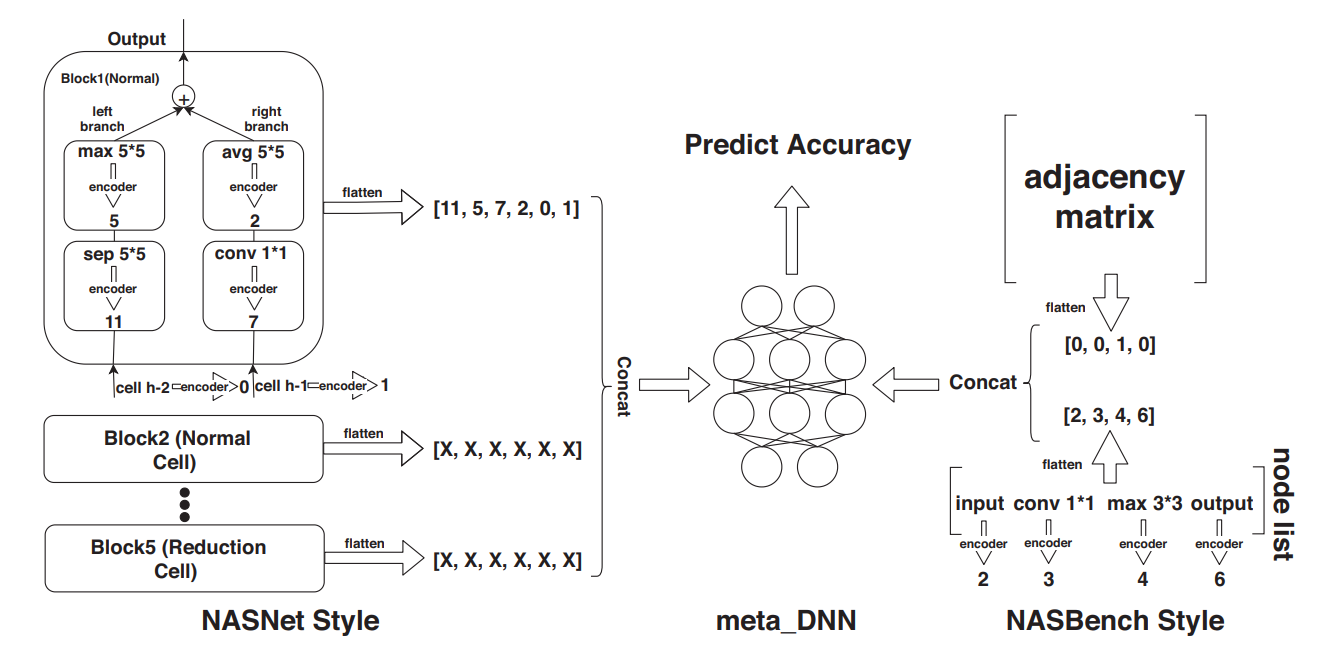
\includegraphics[scale=0.42]{images/nas4.png}
        \caption{Encoding scheme of NASBench and NASNet.}
    \end{figure}
\end{frame}

\begin{frame}{Distributed AlphaX}
\centering 

\begin{figure}
        \centering
        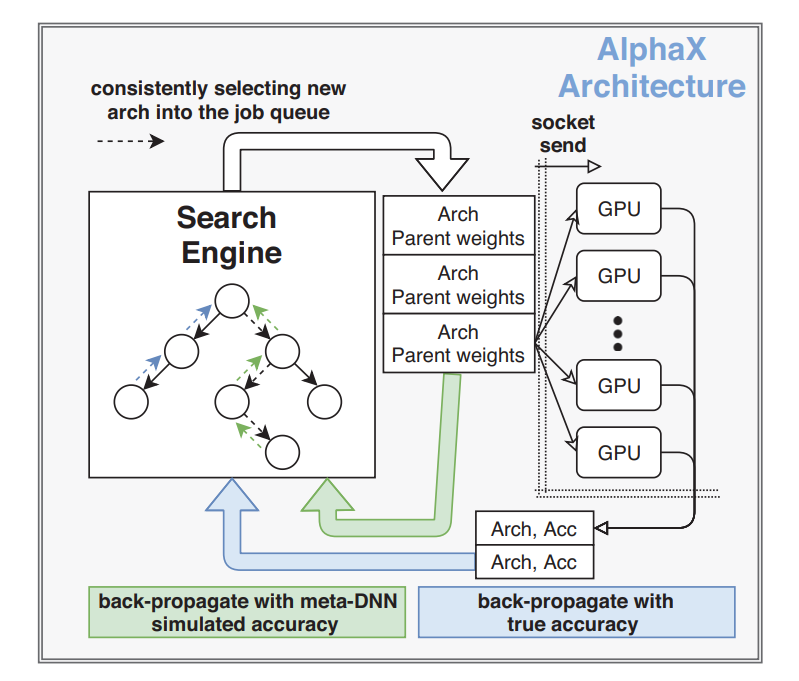
\includegraphics[scale=0.45]{images/nas5.png}
        \caption{Distributed AlphaX: we decouple the original
back-propagation into two parts: one uses predicted accuracy (green arrow), while the other uses the true accuracy
(blue arrow). }
    \end{figure}
 
\end{frame}


\section{Experiments} 
\begin{frame}{Evaluations of architecture search. Open domain search.}
    \begin{figure}
        \centering
        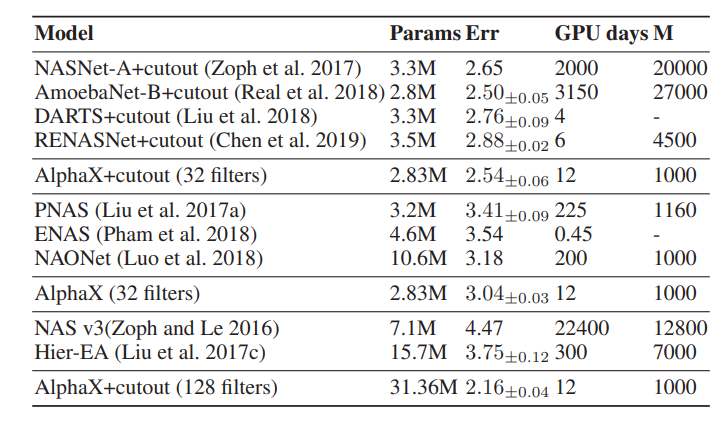
\includegraphics[scale=0.55]{images/nas8.png}
        \caption{The comparisons of our NASNet search results to
other state-of-the-art results on CIFAR-10. M is the number
of sampled architectures in the search.}
    \end{figure}
\end{frame}

\begin{frame}{Evaluations of architecture search. Searching on NAS dataset.}
    \begin{figure}
        \centering
        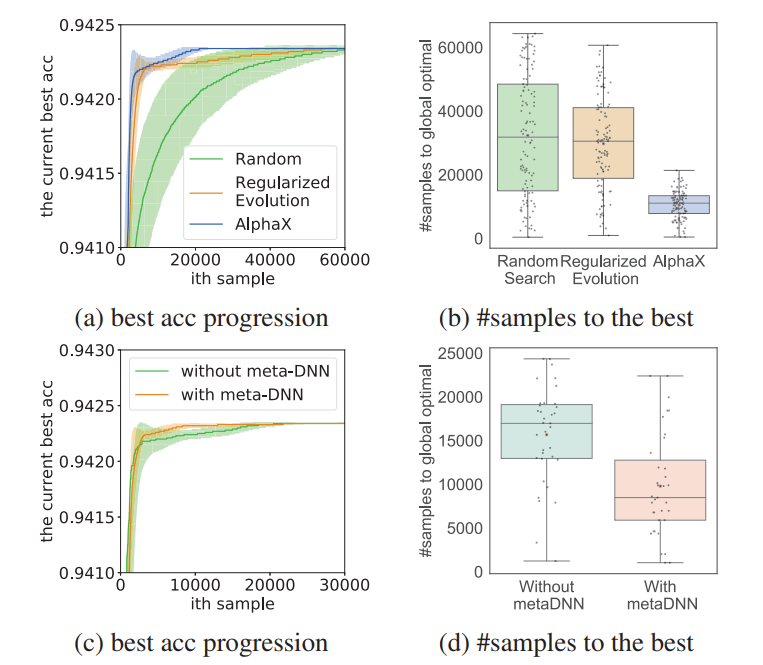
\includegraphics[scale=0.45]{images/nas7.png}
        \caption{Finding the global optimum on NASBench-101:
AlphaX is 3x, 2.8x faster than Random Search and Regularized Evolution on NASBench-101 (nodes ≤ 6).}
    \end{figure}
\end{frame}

\begin{frame}{Evaluations of architecture search. Qualitative evaluations of AlphaX.}
    \begin{figure}
        \centering
        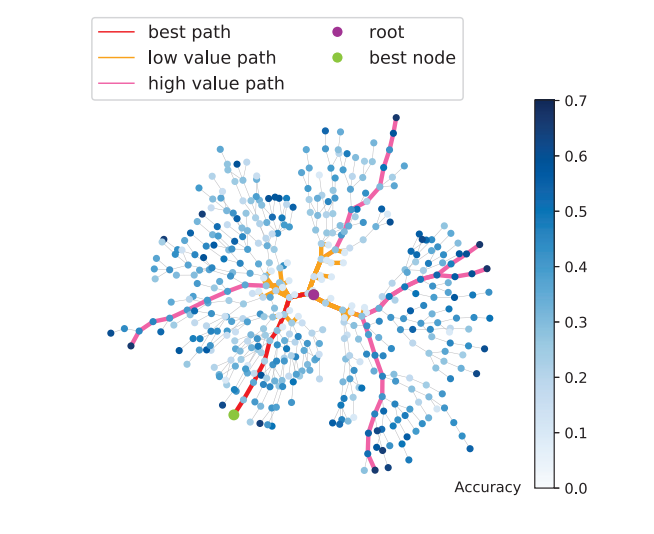
\includegraphics[scale=0.55]{images/nas9.png}
        \caption{ AlphaX search visualization:each node represents
a MCTS state; the node color reflects its value, i.e. accuracy,
indicating how promising a search branch.}
    \end{figure}
\end{frame}

\begin{frame}{Component evaluations. Transfer learning.}
    \begin{figure}
        \centering
        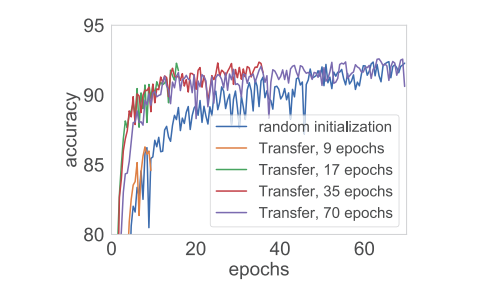
\includegraphics[scale=0.5]{images/nas10.png}
        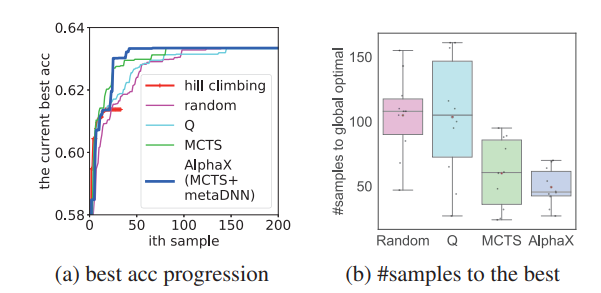
\includegraphics[scale=0.5]{images/nas11.png}
        \caption{\textbf{1.} Validation of transfer learning: transferring
weights significantly reduces the number of epochs in reaching the same accuracy of random initializations (Transfer $17 \to 70$ epochs v.s. random initialization), but insufficient epochs loses accuracy (Transfer, 9 epochs). \textbf{2.} Algorithmic comparisons: AlphaX is consistently the fastest algorithm to reach the global optimal on another
simplified search domain, while Hill Climbing
can easily trap into a local optimal.}
        \label{fig:enter-label}
    \end{figure} 
\end{frame}

\begin{frame}{Algorithm Comparisons}
    \begin{figure}
        \centering
        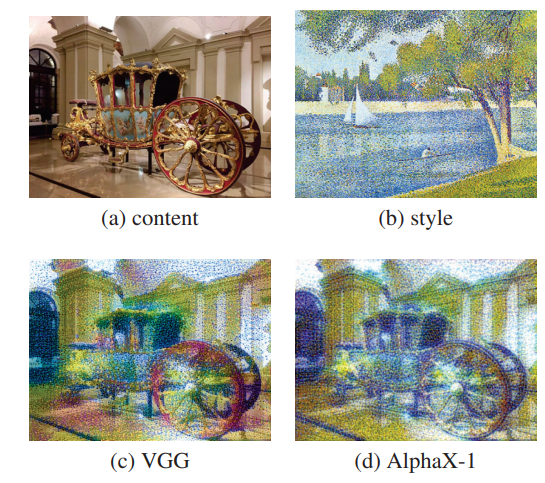
\includegraphics[scale=0.65]{images/nas12.png}
        \caption{Neural Style Transfer: AlphaX-1 v.s. VGG.}
        \label{fig:enter-label}
    \end{figure}
\end{frame}



\begin{frame}{Literature}
    \begin{enumerate}
        \item \textbf{Main article} \href{file:///C:/Users/79267/Downloads/Neural_Architecture_Search_Using_Deep_Neural_Netwo.pdf}
        {Neural Architecture Search Using Deep
Neural Networks and Monte Carlo Tree Search}.
    \end{enumerate}
\end{frame}


\bibliographystyle{unsrt}
\bibliography{sample}
\end{document}